% === Cours de Java
% === Chapitre : La grammaire
\section{La grammaire lexicale de Java}

\leconwithtoc

\subsection{Analyse lexicale}

\begin{frame}{Analyse lexicale de Java}
 Premi�re phase d'analyse d'un programme
\begin{itemize}
\item Examine la s�quence des caract�res d'entr�e
\item Supprime \texttt{caract�res d'espacement} et \texttt{commentaires}
\item Identifie les \textit{tokens} (mots) du langage 
\end{itemize} 
\begin{center}
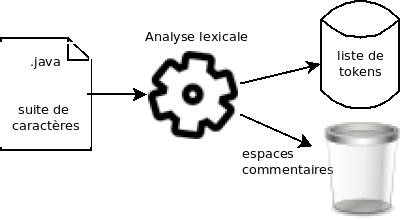
\includegraphics[scale=.5]{../img/phase1} 
\end{center} 
\end{frame}

\begin{frame}{Analyse lexicale de Java}
L'analyse lexicale se base sur une grammaire lexicale
\begin{itemize}
\item Les symboles \texttt{terminaux} sont l'ensemble des caract�res \sigle{Unicode}
\end{itemize} 
\bigskip
\sigle{Java} a fait le choix de l'\sigle{UTF-16} (\sigle{Unicode})
  \begin{itemize}
  \item \sigle{ASCII}: 7 bits
  \item \sigle{ASCII �tendu}: 8 bits
  \item \sigle{EBCDIC}: 8 bits (\sigle{IBM})
  \item \sigle{UTF-16}: 2 bytes, 16 bits 
\\(les 128 premiers caract�res $\equiv$ \sigle{ASCII}) 
  \end{itemize}
\end{frame}

\begin{frame}[fragile]{Les s�quences Unicode}
Java permet une repr�sentation \sigle{ASCII} de tout caract�re \sigle{UTF-16} (via un \textit{caract�re d'�chappement})
\begin{itemize}
\item \emph{Ex} : le caract�re \emph{p} peut aussi s'�crire \code{\u0070} 
\item Une traduction pr�alable est r�alis�e :
\end{itemize}
\begin{Java}
\u0070ublic class MaClasse
\end{Java}
devient
\begin{Java}
public class MaClasse
\end{Java}
\end{frame}

\begin{frame}[fragile]{Les caract�res d'entr�e}
\begin{grammaire}
\nterm{UnicodeInputCharacter} :
   \nterm{UnicodeEscape}
   \nterm{RawInputCharacter}

\nterm{UnicodeEscape} :
   \term{\textbackslash}\nterm{UnicodeMarker} \nterm{HexDigit} \nterm{HexDigit} \nterm{HexDigit} \nterm{HexDigit}

\nterm{UnicodeMarker} :
   \term{u}
   \nterm{UnicodeMarker} \term{u}

\nterm{RawInputCharacter} :
   any Unicode character

\nterm{HexDigit} : one of
   \term{0}  \term{1}  \term{2}  \term{3}  \term{4}  \term{5}  \term{6}  \term{7}  \term{8}  \term{9}    \term{a}  \term{b}  \term{c}  \term{d}  \term{e}  \term{f}     \term{A}  \term{B}  \term{C}  \term{D}  \term{E}  \term{F}  
\end{grammaire}
\end{frame}

\subsection{Les espaces}

\begin{frame}[fragile]{Les caract�res d'espacement}
Les <<espaces>> n'ont pas de sens en \sigle{Java}
\begin{itemize}
\item Peuvent �tre utilis�s librement entre les mots
\item Mais ne peuvent pas couper un mot
\item Exception : les chaines (\textit{String})
\end{itemize}
\begin{grammaire}[basicstyle=\scriptsize]
\nterm{WhiteSpace} :
   the ASCII SP character, also known as "space"
   the ASCII HT character, also known as "horizontal tab"
   the ASCII FF character, also known as "form feed" 
   \nterm{LineTerminator}

\nterm{LineTerminator} :
   the ASCII LF character, also known as "newline"
   the ASCII CR character, also known as "return"
   the ASCII CR character followed by the ASCII LF character
\end{grammaire} 
\end{frame}

\subsection{Les commentaires}

\begin{frame}[fragile]{Le commentaire}
  \begin{itemize}
  \item Sur 1 ligne
    \begin{Java}
// Commentaire sur 1 ligne
    \end{Java}
  \item Sur plusieurs lignes
    \begin{Java}
/* Exemple de commentaire
   sur plusieurs lignes */
    \end{Java}
    \begin{Java}
/** Pour un commentaire Javadoc */
    \end{Java}
  \item Ne peuvent pas �tre imbriqu�s
  \item N'importe o� \textbf{entre} les mots  
  \end{itemize}
\end{frame}

\subsection{Les tokens}

\begin{frame}[fragile]{Les tokens (mots du langage)}
Les caract�res qui restent vont former les \textit{tokens} (mots, symboles terminaux)
\begin{itemize}
\item 5 sortes de tokens 
\begin{grammaire}
\nterm{Token} : one of
    \nterm{Identifier}  \nterm{Literal}  \nterm{Keyword}  \nterm{Separator}  \nterm{Operator}
\end{grammaire}
\end{itemize}
\end{frame}

\begin{frame}[fragile]{Les tokens (mots du langage)}
Liste des \nterm{keyword} (\emph{mots-cl�s} ou r�serv�s)
\begin{grammaire}
\nterm{Keyword} : one of
   \term{abstract}   \term{boolean}   \term{break}   \term{byte}   \term{case}   \term{catch}   
   \term{char} \term{class}   \term{const}   \term{continue}   \term{default}   \term{do}   
   \term{double}   \term{else} \term{extends}   \term{final}   \term{finally}   \term{float}   
   \term{for}   \term{goto}   \term{if} \term{implements}   \term{import}   \term{instanceof}    
   \term{int}   \term{interface} \term{long}   \term{native}   \term{new}   \term{package}   
   \term{private}   \term{protected} \term{public}   \term{return}   \term{short}   
   \term{static}  \term{super}   \term{switch} \term{synchronized}  \term{this}   \term{throw}   
   \term{throws}   \term{transient} \term{try}   \term{void}   \term{volatile}   \term{while}
\end{grammaire}
\end{frame}

\begin{frame}[fragile]{Les tokens (mots du langage)}
Les identifiants
\begin{grammaire}
\nterm{Identifier} :
   \nterm{IdentifierChars} 
         but not a \nterm{Keyword} or \nterm{BooleanLitteral} or \nterm{NullLitteral}

\nterm{IdentifierChars} :
   \nterm{JavaLetter} 
   \nterm{IdentifierChars} \nterm{JavaLetterOrDigit}

\nterm{JavaLetter} :
   any Unicode character that is a Java letter (_ et \$ sont compris)

\nterm{JavaLetterOrDigit} :
   any Unicode character that is a Java letter-or-digit 
\end{grammaire}
(cf. la grammaire compl�te pour les d�tails)
\end{frame}

\begin{frame}[fragile]{Les tokens (mots du langage)}
Liste des s�parateurs et op�rateurs
\begin{grammaire}
\nterm{Separator} : one of
    \term{(}  \term{)}  \term{\{}  \term{\}}  \term{[}  \term{]}  \term{;}  \term{,}  \term{.}

\nterm{Operator} : one of
    \term{=}   \term{>}   \term{<}   \term{!}   \term{~}   \term{?}   \term{:}  \term{==}   \term{<=}   \term{>=}   \term{!=}   \term{&&}   \term{||}   
    \term{++}   \term{--}   \term{+}   \term{-}   \term{*}   \term{/}   \term{&}   \term{|}   \term{^}   \term{%}   \term{<<}   \term{>>}   \term{>>>}
    \term{+=}   \term{-=}   \term{*=}   \term{/=}   \term{&=}   \term{|=}   \term{^=}   \term{%=}   \term{<<=}   \term{>>=}   \term{>>>=}
\end{grammaire}
Comment l'analyseur lexical va-t-il reconnaitre \java|---| ?
\end{frame}

\begin{frame}{R�capitulatif des phases de compilation}
Une fois les tokens identifi�s, le compilateur peut passer � l'analyse syntaxique et s�mantique
\begin{center}
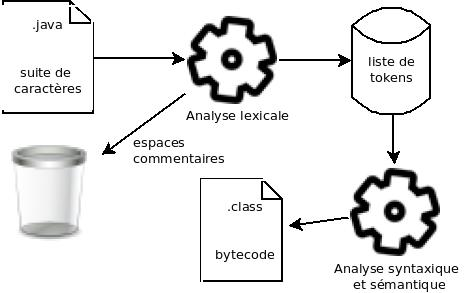
\includegraphics[scale=.5]{../img/phases} 
\end{center} 
\end{frame}

